\PassOptionsToPackage{unicode=true}{hyperref} % options for packages loaded elsewhere
\PassOptionsToPackage{hyphens}{url}
\documentclass[11pt,dvipsnames,ignorenonframetext,aspectratio=169]{beamer}
\IfFileExists{pgfpages.sty}{\usepackage{pgfpages}}{}
\setbeamertemplate{caption}[numbered]
\setbeamertemplate{caption label separator}{: }
\setbeamercolor{caption name}{fg=normal text.fg}
\beamertemplatenavigationsymbolsempty
\usepackage{lmodern}
\usepackage{amssymb,amsmath}
\usepackage{ifxetex,ifluatex}
\usepackage{fixltx2e} % provides \textsubscript
\ifnum 0\ifxetex 1\fi\ifluatex 1\fi=0 % if pdftex
  \usepackage[T1]{fontenc}
  \usepackage[utf8]{inputenc}
\else % if luatex or xelatex
  \ifxetex
    \usepackage{mathspec}
  \else
    \usepackage{fontspec}
\fi
\defaultfontfeatures{Ligatures=TeX,Scale=MatchLowercase}







\fi

  \usetheme[]{monash}

  \usecolortheme{monashwhite}


% A default size of 24 is set in beamerthememonash.sty
  \setbeamerfont{title}{series=\bfseries,parent=structure,size=\fontsize{18pt}{32}}

% Title page
\setbeamertemplate{title page}
{\placefig{-0.01}{-0.01}{width=1.01\paperwidth,height=1.01\paperheight}{fusrekhola\_falls\_kaski\_20210814.jpg}
\begin{textblock}{7.5}(1,2.8)\usebeamerfont{title}
{\color{white}\raggedright\par\inserttitle}
\end{textblock}
\begin{textblock}{7.5}(1,7)
{\color{white}\raggedright{\insertauthor}\mbox{}\\[0.2cm]
\insertdate}
\end{textblock}}


  \useinnertheme{rounded}

  \useoutertheme{smoothtree}

% use upquote if available, for straight quotes in verbatim environments
\IfFileExists{upquote.sty}{\usepackage{upquote}}{}
% use microtype if available
\IfFileExists{microtype.sty}{%
  \usepackage{microtype}
  \UseMicrotypeSet[protrusion]{basicmath} % disable protrusion for tt fonts
}{}


\newif\ifbibliography


\hypersetup{
      pdftitle={Defence mechanisms against pathogens, parasites, insects},
            colorlinks=true,
    linkcolor=red,
    citecolor=Blue,
    urlcolor=lightgrayd,
    breaklinks=true}
%\urlstyle{same}  % Use monospace font for urls







% Prevent slide breaks in the middle of a paragraph:
\widowpenalties 1 10000
\raggedbottom

  \AtBeginPart{
    \let\insertpartnumber\relax
    \let\partname\relax
    \frame{\partpage}
  }
  \AtBeginSection{
    \ifbibliography
    \else
      \let\insertsectionnumber\relax
      \let\sectionname\relax
      \frame{\sectionpage}
    \fi
  }
  \AtBeginSubsection{
    \let\insertsubsectionnumber\relax
    \let\subsectionname\relax
    \frame{\subsectionpage}
  }



\setlength{\parindent}{0pt}
\setlength{\parskip}{6pt plus 2pt minus 1pt}
\setlength{\emergencystretch}{3em}  % prevent overfull lines
\providecommand{\tightlist}{%
  \setlength{\itemsep}{0pt}\setlength{\parskip}{0pt}}

  \setcounter{secnumdepth}{0}


%% Monash overrides
\AtBeginSection[]{
   \frame<beamer>{
   \frametitle{Outline}\vspace*{0.2cm}
   
   \tableofcontents[currentsection,hideallsubsections]
  }}

% Redefine shaded environment if it exists (to ensure text is black)
\ifcsname Shaded\endcsname
  \definecolor{shadecolor}{RGB}{225,225,225}
  \renewenvironment{Shaded}{\color{black}\begin{snugshade}\color{black}}{\end{snugshade}}
\fi
%%

\newlength{\cslhangindent}
\setlength{\cslhangindent}{1.5em}
\newenvironment{CSLReferences}%
  {}%
  {\par}

  \usepackage{setspace}
  \usepackage{wasysym}
  % \usepackage{footnote} % don't use this this breaks all
  \usepackage{fontenc}
  \usepackage{fontawesome}
  \usepackage{booktabs,siunitx}
  \usepackage{longtable}
  \usepackage{array}
  \usepackage{multirow}
  \usepackage{wrapfig}
  \usepackage{float}
  \usepackage{colortbl}
  \usepackage{pdflscape}
  \usepackage{tabu}
  \usepackage{threeparttable}
  \usepackage{threeparttablex}
  \usepackage[normalem]{ulem}
  \usepackage{makecell}
  \usepackage{xcolor}
  \usepackage{tikz} % required for image opacity change
  \usepackage[absolute,overlay]{textpos} % for text formatting
  \usepackage{chemfig}
  \usepackage[skip=0.333\baselineskip]{caption}
  % \newcommand*{\AlignChar}[1]{\makebox[1ex][c]{\ensuremath{\scriptstyle#1}}}%
  \usepackage{siunitx}

  % this font option is amenable for beamer
  \setbeamerfont{caption}{size=\tiny}
  \singlespacing
  \definecolor{lightgrayd}{gray}{0.95}
  \definecolor{skyblued}{rgb}{0.65, 0.6, 0.94}
  \definecolor{oranged}{RGB}{245, 145, 200}

  % % better to insert it into template itself
  % \newlength{\cslhangindent}
  % \setlength{\cslhangindent}{1.5em}
  % \newenvironment{cslreferences}%
  %   {\setlength{\parindent}{0pt}%
  %   \everypar{\setlength{\hangindent}{\cslhangindent}}\ignorespaces}%
  %   {\par}

  \usepackage[caption=false]{subfig}

  \newcommand{\bcolumns}{\begin{columns}[T, onlytextwidth]}
  \newcommand{\ecolumns}{\end{columns}}

  \newcommand{\bdescription}{\begin{description}}
  \newcommand{\edescription}{\end{description}}

  \newcommand{\bitemize}{\begin{itemize}}
  \newcommand{\eitemize}{\end{itemize}}
  \AtBeginSubsection{}

  \title[]{Defence mechanisms against pathogens, parasites, insects}


  \author[
        \vspace{-0.5cm}Deependra Dhakal\\
Assistant Professor\\
Agriculture and Forestry University\\
\textit{ddhakal.rookie@gmail.com}\\
\url{https://rookie.rbind.io}
    ]{\vspace{-0.5cm}Deependra Dhakal\\
Assistant Professor\\
Agriculture and Forestry University\\
\textit{ddhakal.rookie@gmail.com}\\
\url{https://rookie.rbind.io}}


\date[
      
  ]{
    }

\begin{document}

% Hide progress bar and footline on titlepage
  \begin{frame}[plain]
  \titlepage
  \end{frame}


   \frame<beamer>{
   \frametitle{Outline}\vspace*{0.2cm}
   
   \tableofcontents[hideallsubsections]
  }

\hypertarget{defense-mechanisms-against-pathogens-parasites}{%
\section{Defense mechanisms against pathogens,
parasites}\label{defense-mechanisms-against-pathogens-parasites}}

\begin{frame}{}
\protect\hypertarget{section}{}
\begin{itemize}
\tightlist
\item
  Genetic information (determines the form and function) is encoded as
  DNA or (exceptionally) RNA.

  \begin{itemize}
  \tightlist
  \item
    Nucleus
  \item
    Mitochondria
  \item
    Plasmid (autonomously replicating)
  \item
    Chloroplasts
  \end{itemize}
\item
  A gene (in general) is characterized by:

  \begin{itemize}
  \tightlist
  \item
    100-500 codon triplets
  \item
    Coding and and non-coding region
  \item
    Protein or RNA as code product
  \end{itemize}
\item
  Genetic processes

  \begin{itemize}
  \tightlist
  \item
    Replication
  \item
    Transcription
  \item
    Translation
  \item
    Regulatory elements -- promoters, enhancers, silencers or
    terminators
  \end{itemize}
\end{itemize}
\end{frame}

\hypertarget{mechanisms-of-infection}{%
\section{Mechanisms of infection}\label{mechanisms-of-infection}}

\begin{frame}{}
\protect\hypertarget{section-1}{}
\begin{figure}
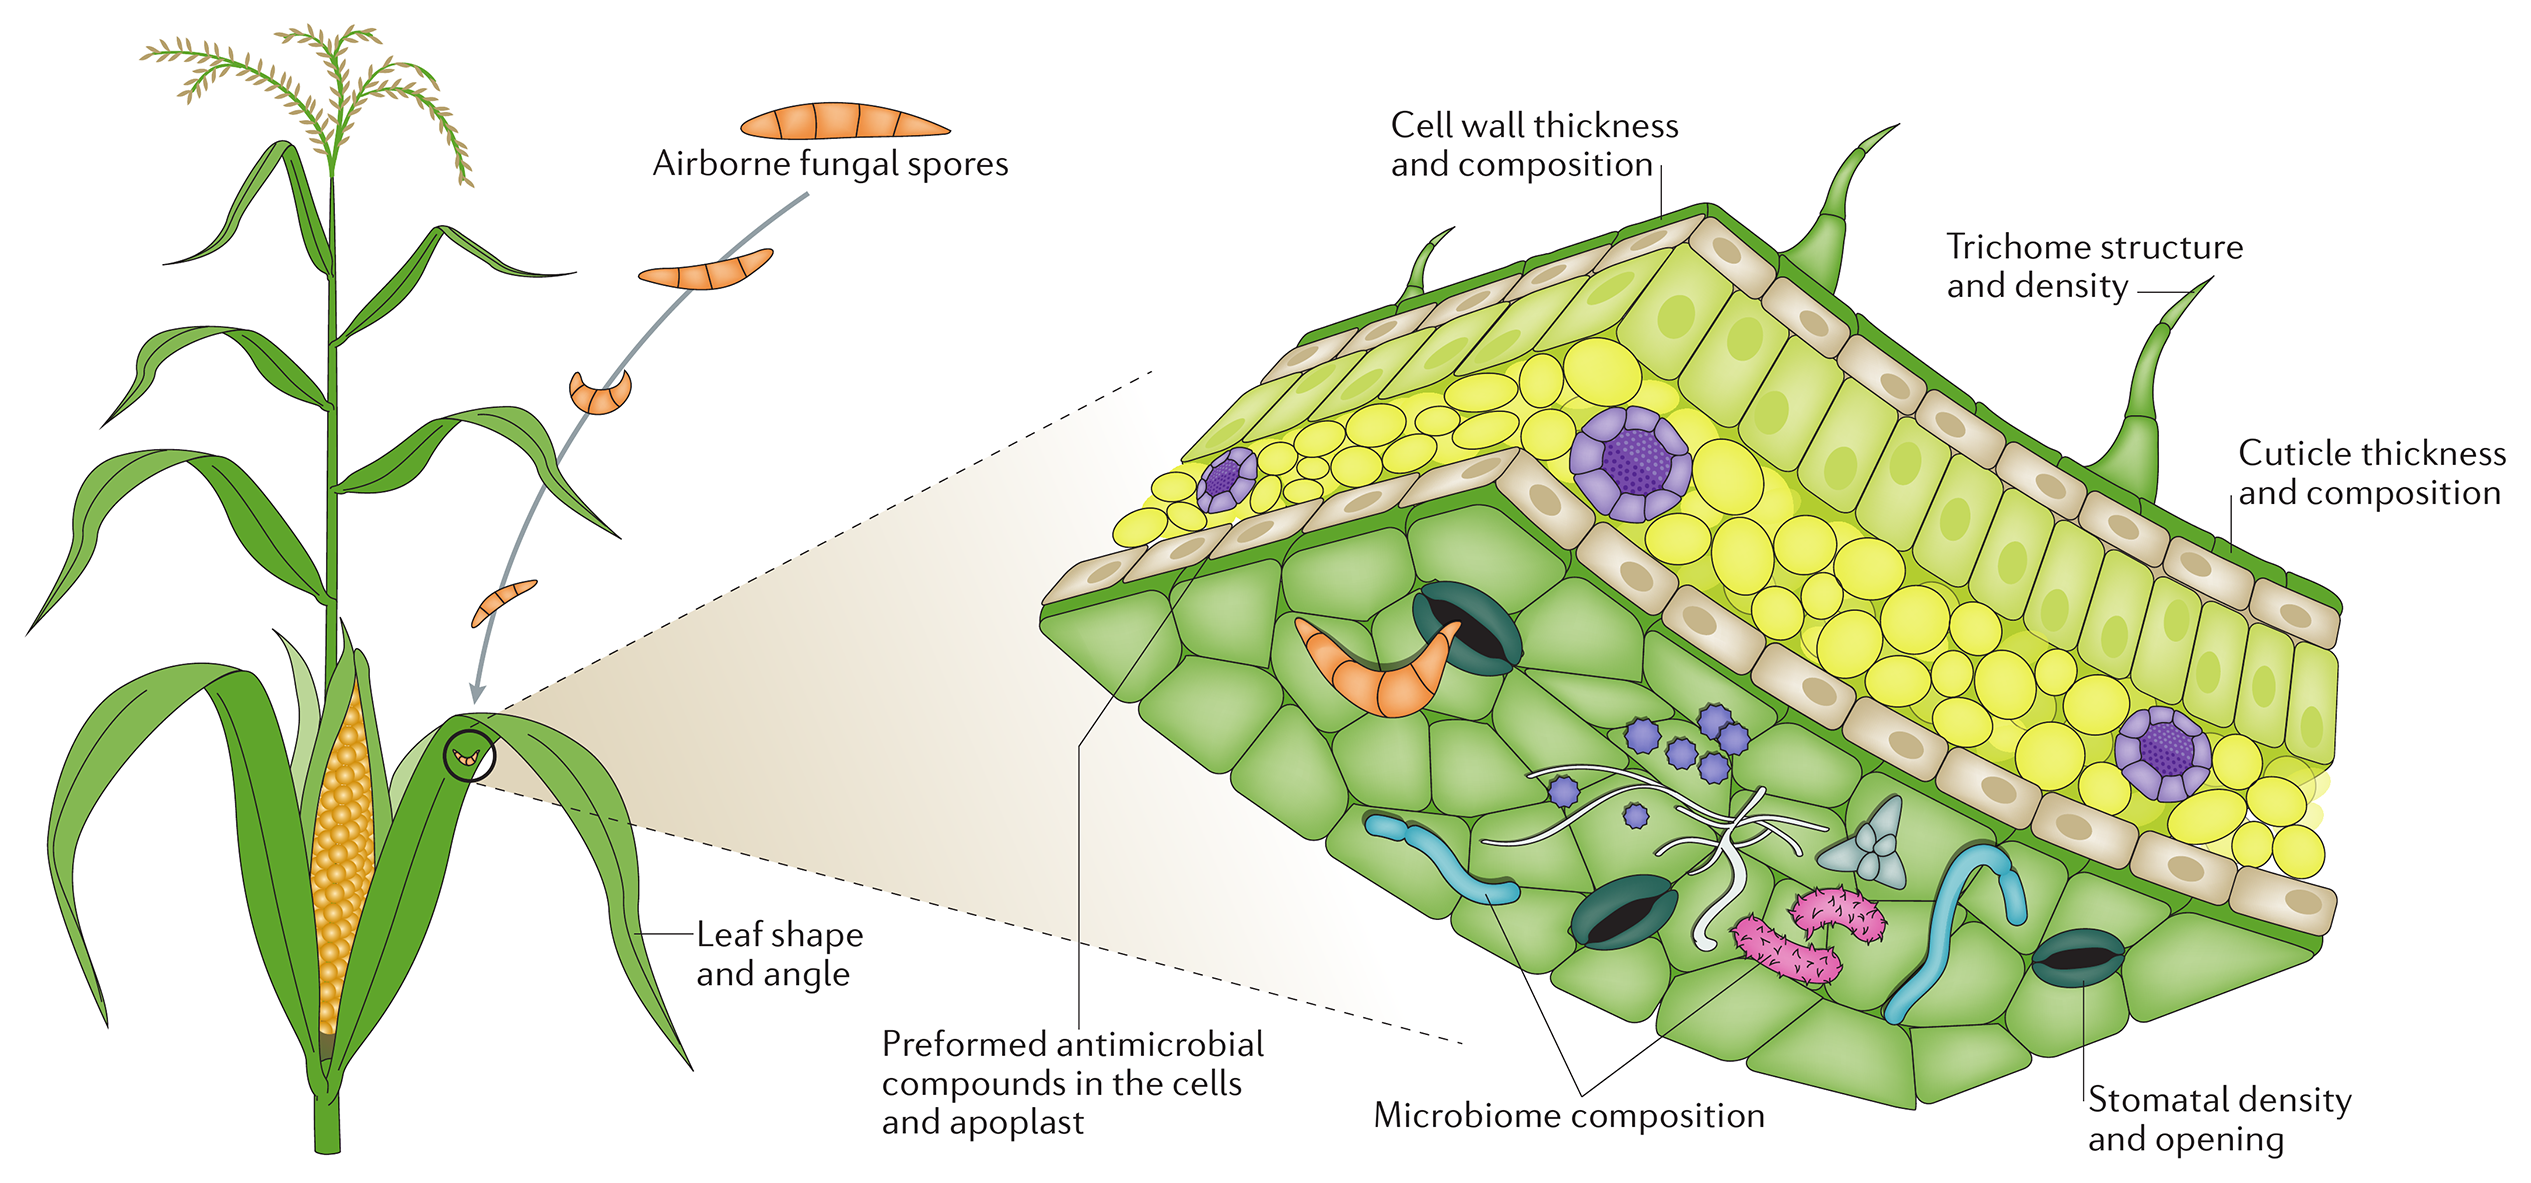
\includegraphics[width=0.8\linewidth]{../images/infection_process_plants_extracellular} \caption{Resistance mechanisms at the tissue level. At the organismal and tissue levels, the success of a pathogen can be influenced by a range of features of the morphology, biochemistry and microbiome of the plant.}\label{fig:infection-mechanism-extracellular}
\end{figure}
\end{frame}

\begin{frame}{}
\protect\hypertarget{section-2}{}
\begin{figure}
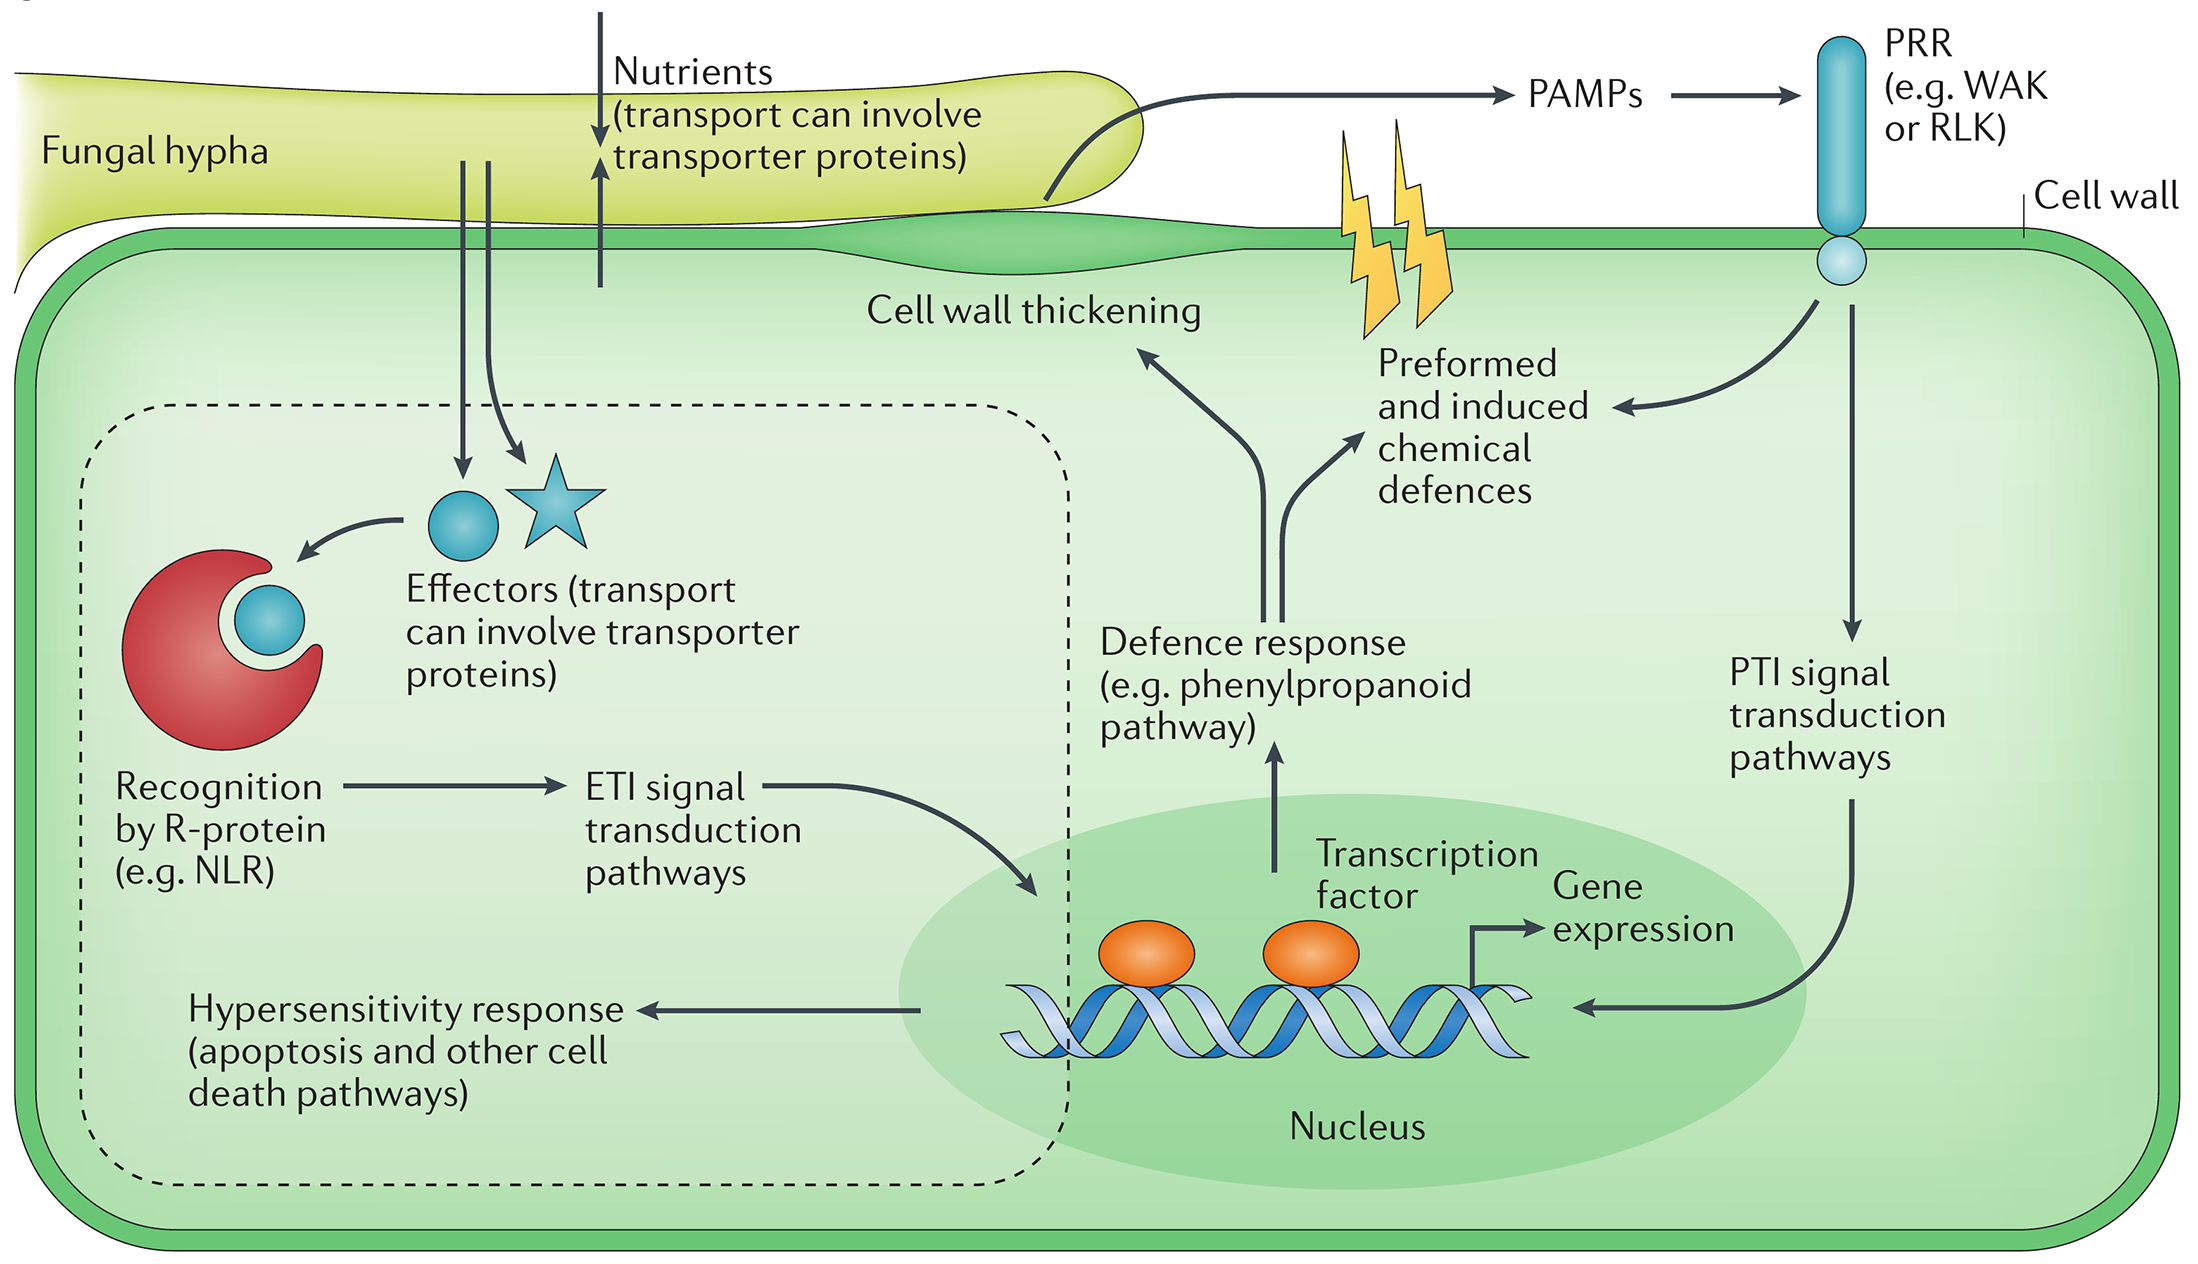
\includegraphics[width=0.8\linewidth]{../images/infection_process_plants_intracellular} \caption{At cellular level, factors that affect the ability of a pathogen to infect its plant host include defence responses triggered by recognition events in the host via PRRs, such as WAKs or RLKs, and resistance proteins (R-proteins), such as NLR proteins, nutrient availability in the apoplast and cytoplasm; pre-existing chemical factors; and cell wall constitution. These factors are affected by host genotype and are potential causes of quantitative variation. Qualitative variation in resistance usually, though not always, occurs at the level of resistance gene-effector interactions.}\label{fig:infection-mechanism-intracellular}
\end{figure}
\end{frame}

\begin{frame}{Genetic processes involved in infection}
\protect\hypertarget{genetic-processes-involved-in-infection}{}
\begin{figure}

{\centering 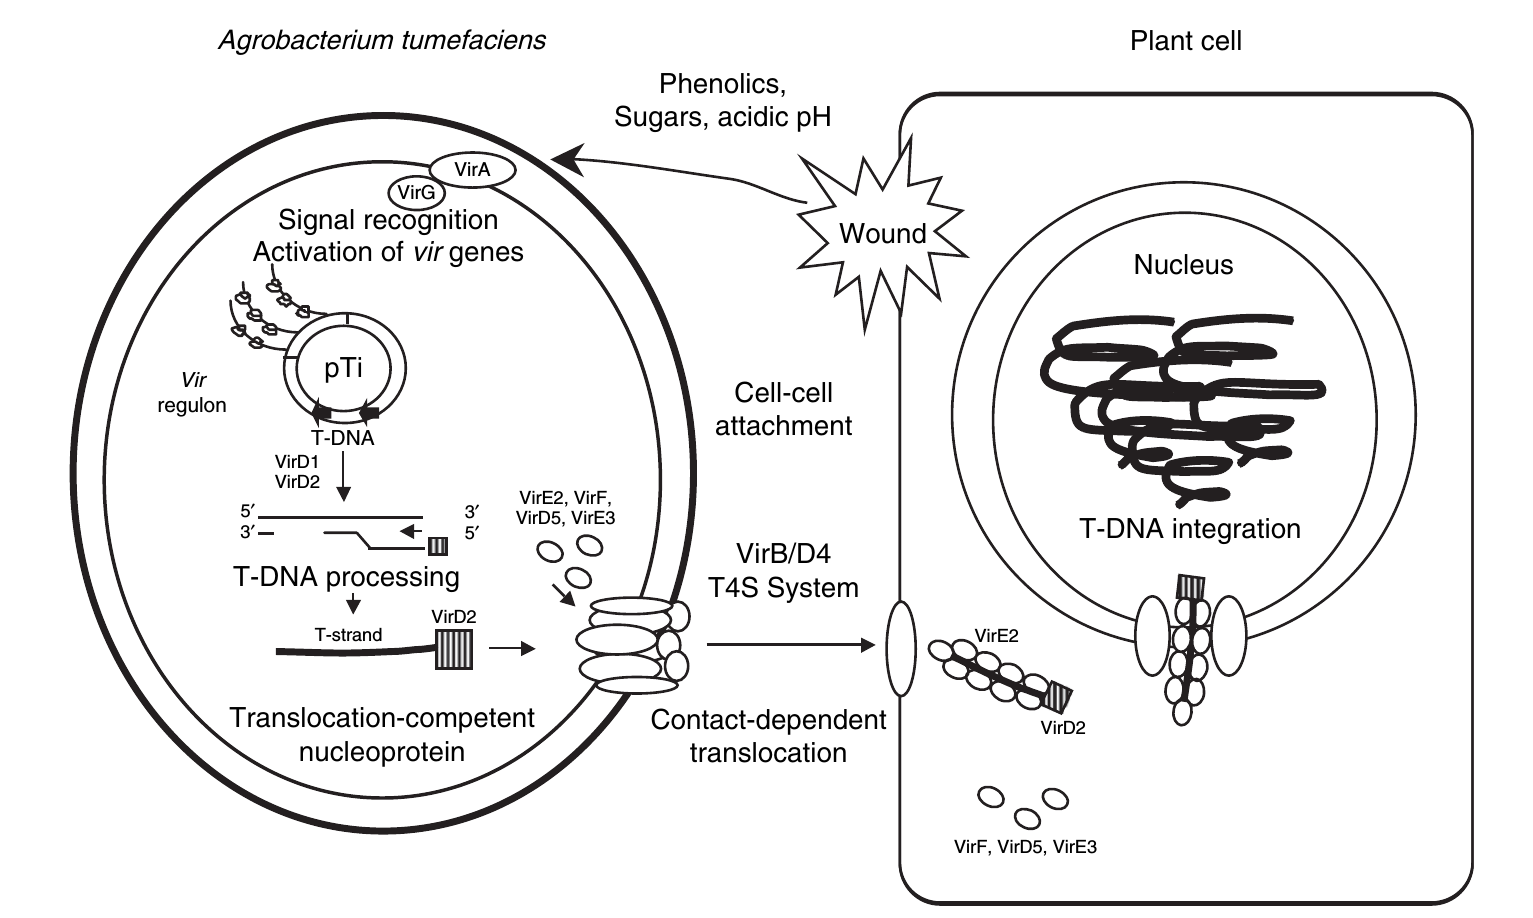
\includegraphics[width=0.66\linewidth]{../images/agrobacterium-transformation} 

}

\caption{Overview of agrobacterium tumefaciens infection process. Upon activation of the VirA/VirG two-component signal transduction system by signals released from wounded plant cells, a single-strand transferred DNA (T-DNA) is processed from the Ti plasmid and delivered as a nucleoprotein complex (T-complex) to plant nuclei. Expression of T-DNA genes in the plant result in the loss of cell growth control and tumor formation.}\label{fig:mechanism-of-infection}
\end{figure}
\end{frame}

\begin{frame}{Mechanisms of genetic resistance (Van Esse, Reuber, and
Does 2020)}
\protect\hypertarget{mechanisms-of-genetic-resistance-van2020genetic}{}
\begin{center}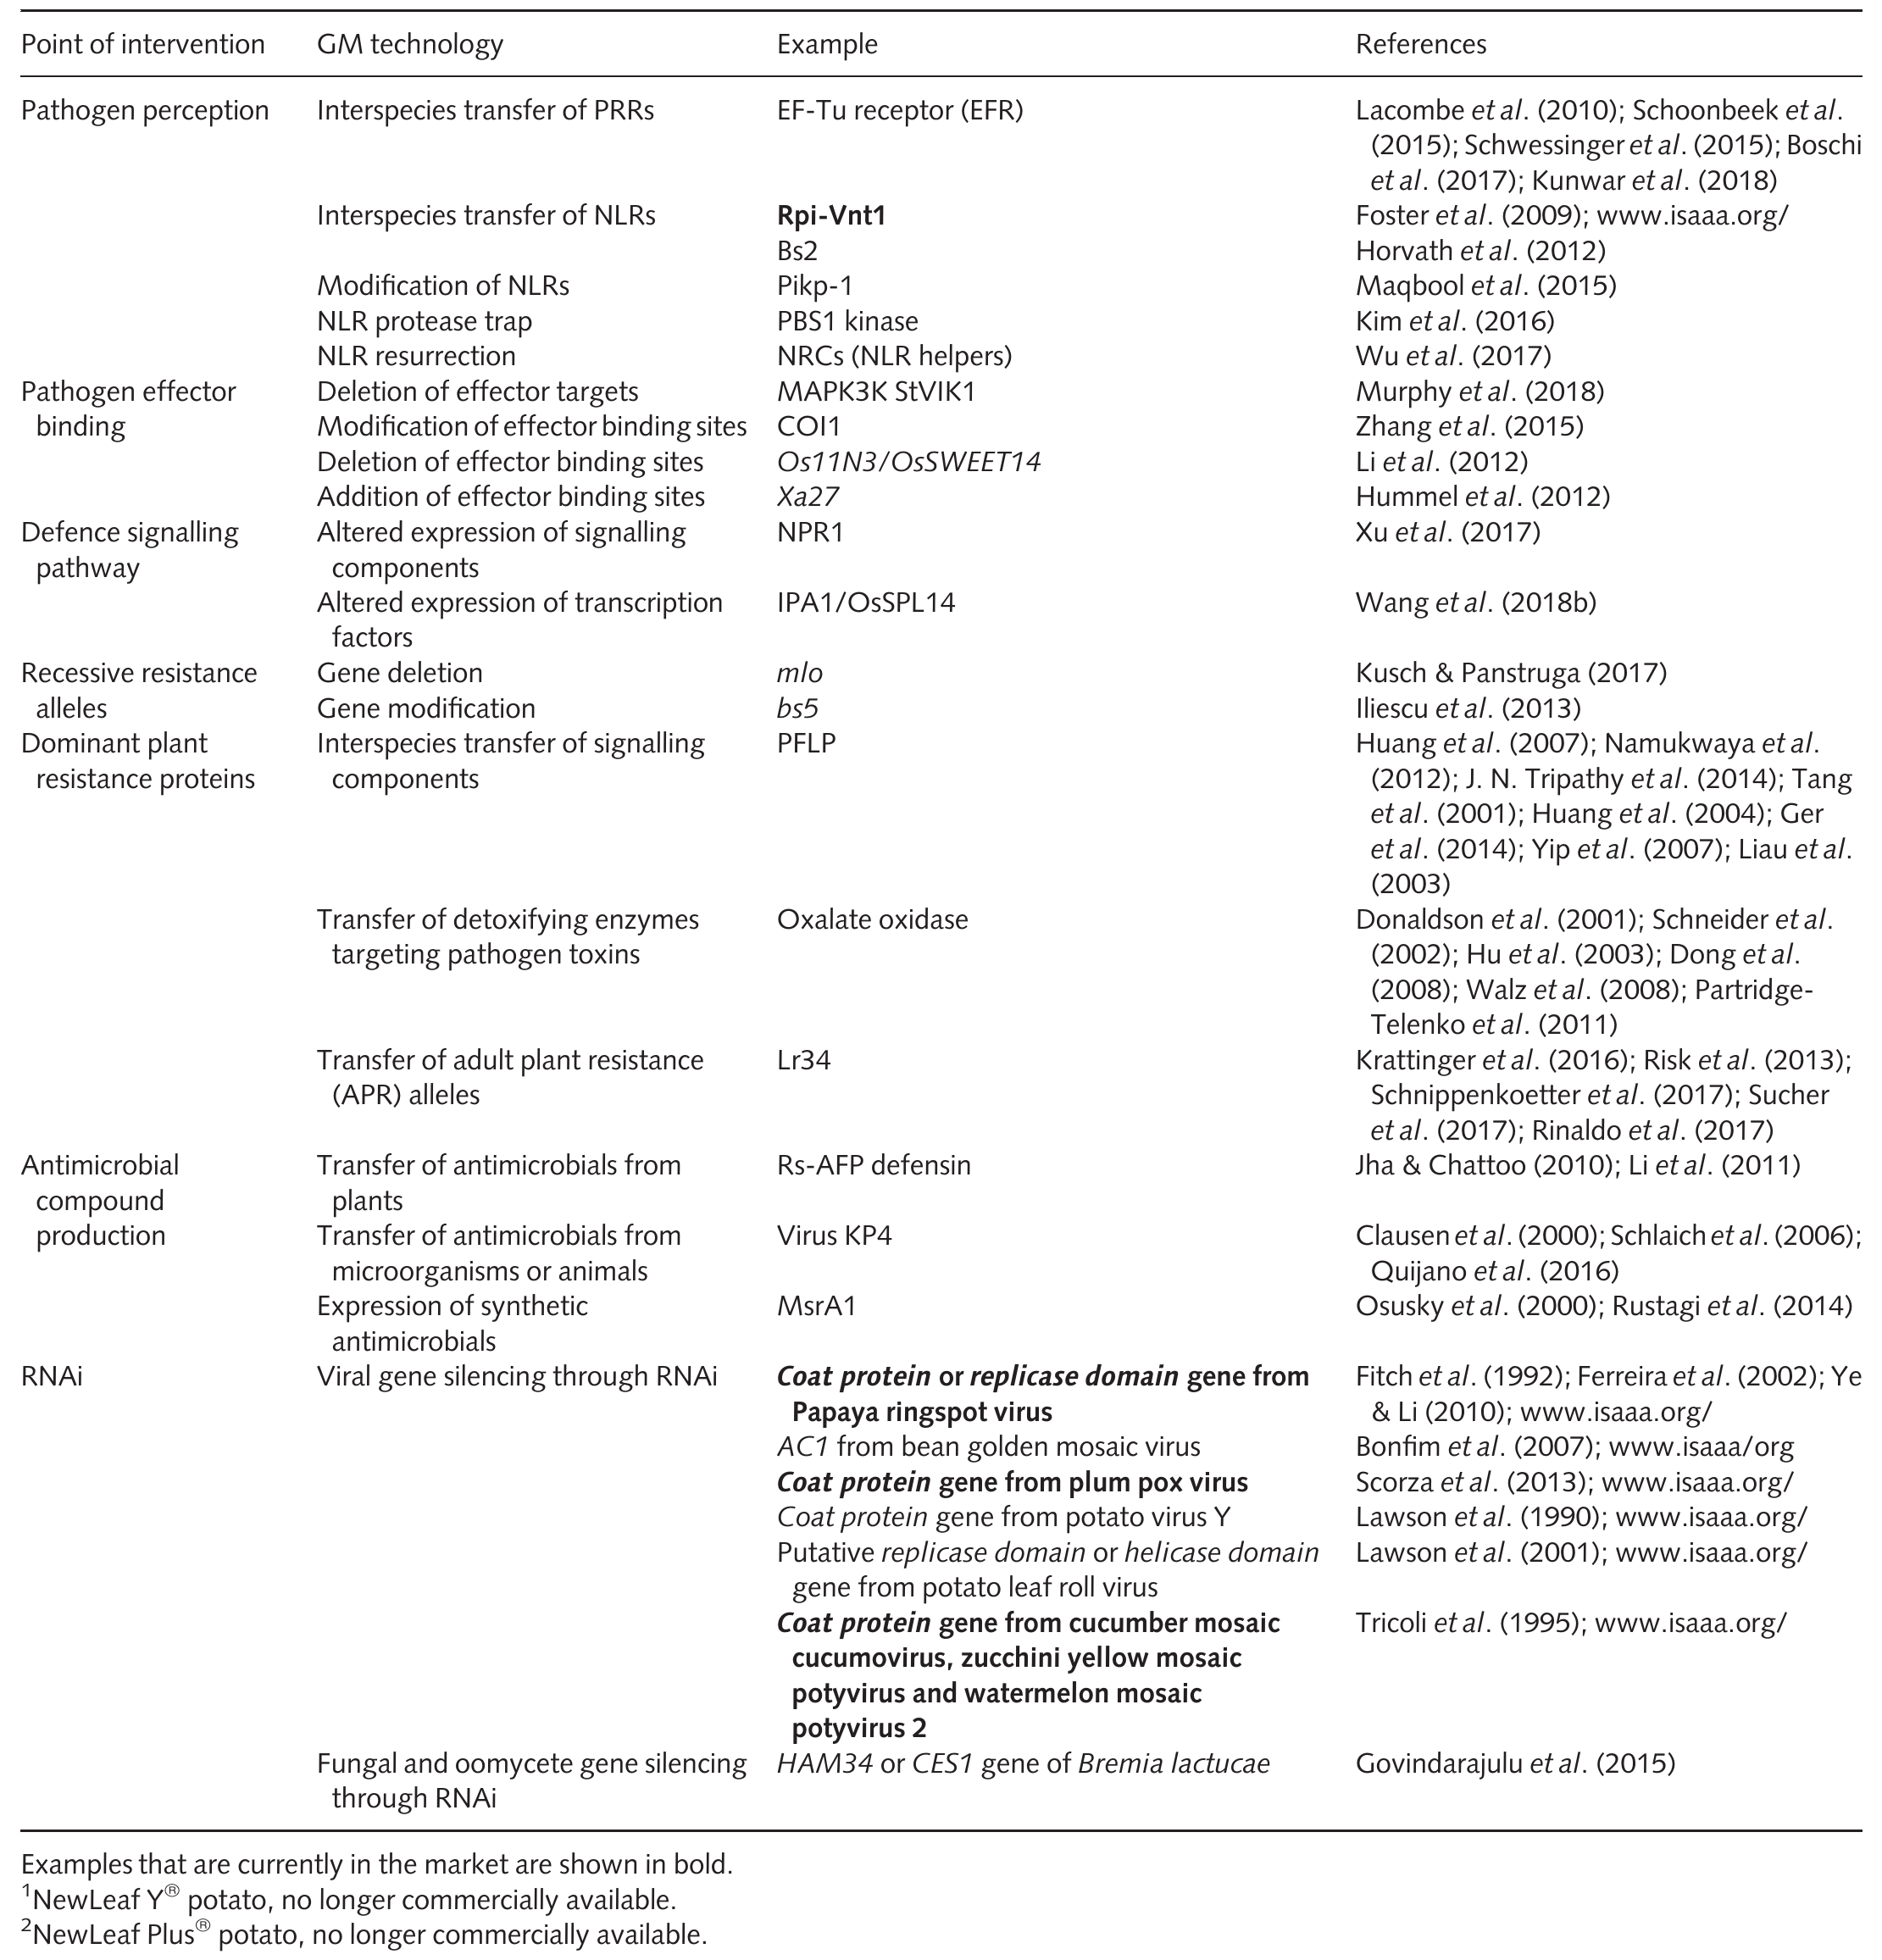
\includegraphics[width=0.4\linewidth]{../images/genetic_solution_pathogens} \end{center}
\end{frame}

\hypertarget{gene-for-gene-hypothesis}{%
\section{Gene for gene hypothesis}\label{gene-for-gene-hypothesis}}

\begin{frame}{}
\protect\hypertarget{section-3}{}
\begin{itemize}
\tightlist
\item
  Flor (1956) was the first to show there was a `gene-for-gene'
  relationship between the pathogen's avirulence ( \emph{Avr}) genes and
  the resistance ( \emph{R}) genes of its host.
\end{itemize}
\end{frame}

\hypertarget{defense-mechanisms-against-insects}{%
\section{Defense mechanisms against
insects}\label{defense-mechanisms-against-insects}}

\hypertarget{bibliography}{%
\section{Bibliography}\label{bibliography}}

\begin{frame}{References}
\protect\hypertarget{references}{}
\hypertarget{refs}{}
\begin{CSLReferences}{1}{0}
\leavevmode\vadjust pre{\hypertarget{ref-flor1956complementary}{}}%
Flor, HH. 1956. {``The Complementary Genic Systems in Flax and Flax
Rust.''} \emph{Advances in Genetics} 8: 29--54.

\leavevmode\vadjust pre{\hypertarget{ref-van2020genetic}{}}%
Van Esse, H Peter, T Lynne Reuber, and Dieuwertje van der Does. 2020.
{``Genetic Modification to Improve Disease Resistance in Crops.''}
\emph{New Phytologist} 225 (1): 70--86.

\end{CSLReferences}
\end{frame}




\end{document}
